\documentclass[onecolumn, draftclsnofoot,10pt, compsoc]{IEEEtran}
\usepackage{graphicx}
\usepackage{url}
\usepackage{setspace}
\usepackage{pgfgantt}
\usepackage{geometry}
\geometry{textheight=9.5in, textwidth=7in}


% 1. Fill in these details
\def \CapstoneTeamName{		Team Sandy}
\def \CapstoneTeamNumber{		44}
\def \GroupMemberOne{			Andrew Soltesz}
\def \GroupMemberTwo{			Mark Sprouse}
\def \GroupMemberThree{			Raja Petroff}
\def \CapstoneProjectName{		AR Sandbox for Construction Planning}
\def \CapstoneSponsorCompany{	Oregon State University}
\def \CapstoneSponsorPerson{		Dr. Joseph Louis}

% 2. Uncomment the appropriate line below so that the document type works
\def \DocType{		%Problem Statement
				Requirements Document
				%Technology Review
				%Design Document
				%Progress Report
				}
			
\newcommand{\NameSigPair}[1]{\par
\makebox[2.75in][r]{#1} \hfil 	\makebox[3.25in]{\makebox[2.25in]{\hrulefill} \hfill		\makebox[.75in]{\hrulefill}}
\par\vspace{-12pt} \textit{\tiny\noindent
\makebox[2.75in]{} \hfil		\makebox[3.25in]{\makebox[2.25in][r]{Signature} \hfill	\makebox[.75in][r]{Date}}}}
% 3. If the document is not to be signed, uncomment the RENEWcommand below
%\renewcommand{\NameSigPair}[1]{#1}

%%%%%%%%%%%%%%%%%%%%%%%%%%%%%%%%%%%%%%%
\begin{document}
\begin{titlepage}
    \pagenumbering{gobble}
    \begin{singlespace}
    	%
\includegraphics[height=4cm]{coe_v_spot1}
        \hfill 
        % 4. If you have a logo, use this includegraphics command to put it on the coversheet.
        %\includegraphics[height=4cm]{CompanyLogo}   
        \par\vspace{.2in}
        \centering
        \scshape{
            \huge CS Capstone \DocType \par
            {\large\today}\par
            \vspace{.5in}
            \textbf{\Huge\CapstoneProjectName}\par
            \vfill
            {\large Prepared for}\par
            \Huge \CapstoneSponsorCompany\par
            \vspace{5pt}
            {\Large\NameSigPair{\CapstoneSponsorPerson}\par}
            {\large Prepared by }\par
            Group\CapstoneTeamNumber\par
            % 5. comment out the line below this one if you do not wish to name your team
            \CapstoneTeamName\par 
            \vspace{5pt}
            {\Large
                \NameSigPair{\GroupMemberOne}\par
                \NameSigPair{\GroupMemberTwo}\par
                \NameSigPair{\GroupMemberThree}\par
            }
            \vspace{20pt}
        }
        \begin{abstract}
        % 6. Fill in your abstract    
        	This document outlines the functionality of the AR Sandbox for Construction Planning Project.  This project consists of a sandbox which will have various images and information projected onto it.  This information may be modified from a computer terminal, but is always dependent on the height of the sand.  This information will range from visual representations of the height to calculations on the construction costs of moving through the terrain.
        \end{abstract}     
    \end{singlespace}
\end{titlepage}
\newpage
\pagenumbering{arabic}
\tableofcontents
% 7. uncomment this (if applicable). Consider adding a page break.
%\listoffigures
%\listoftables
\clearpage

% 8. now you write!
%rank by necessity:
%Essential: lack of these features is unacceptable to the client
%conditional: would enhance product but absence would not make it unacceptable to the client
%optional: stretch goals

%\section{Functionality}
%What is the software supposed to do?

%\section{External Interfaces}
%How does the software interact with people, the system's hardware, other hardware, and software?

%\section{Performance}
%What is the speed, availability, response time, recovery time of the various software functions?

%\section{Attributes}
%What are the portability, correctness, maintainability, security, etc. considerations? 

%\section{Design Constraints}
%Are there any required standards in effect, implementation language, policies for database integrity, resource limits, operating environments, etc.?

%see section 5 of IEEE std 830-1998 for description of sections
\section{Introduction}
\subsection{Purpose}
The purpose of this requirements document is to outline what our product, the AR sandbox, will do and what is required for it to function.
\par The intended audience of the requirements document is the client, our instructors, and any future students or engineers that wish to implement our product.
\subsection{Scope}
The product to be produced is an interactive augmented reality (AR) sandbox. The software for this AR Sandbox will be used to create an extensible system that will enable the development of applications within the Civil and Construction Engineering domain.  For demonstration purposes, our project focuses on the development of an application that allows for topographical overlays along with cut \& fill analytics represented.
\par The objective of the software is to provide an intuitive means of calculating and representing cut \& fill sections along a highway during its construction phase.  This will enable engineers to collaborate, plan, communicate, and learn about these civil concepts in an alternate manner.
\subsection{Definitions, Acronyms, and Abbreviations}
\begin{itemize}
\item AR Sandbox: Augmented reality sandbox. A physical sandbox with a depth sensor and projector that displays graphics on the sand, such as roadways and ground topology.
\item Augmented Reality: A way of mixing computer images with the user's vision. This refers to the graphics displayed over the sand. When a user manipulates the sand, the graphics displayed on the sand will change.
\item Projection: The image cast on the sand's surface by the projector
\item Depth Sensor: A digital imaging device which uses a grayscale image to represent the distance from the sensor to the nearest surface.
\end{itemize}
\subsection{References}
Original UC Davis AR Sandbox: https://arsandbox.ucdavis.edu/
\subsection{Overview}
The rest of this requirements document describes what our product is and what it is supposed to do. It describes the functionality and necessary constraints, such as the hardware required. It also describes performance metrics, design constraints, and lastly, stretch goals, which we will fulfill if enough time remains after the original requirements are fulfilled.
\par The requirements document is organized into three sections. The first section describes the product and gives an overview of the whole document. The second section gives a broad description of the product and its requirements; however, it does not describe specific requirements. The third section defines the actual requirements of the product.

\section{Overall Description} 
\subsection{Product Perspective}
The augmented reality sandbox is a self-contained system. The majority of user interaction occurs on the surface of the sand itself. 
Certain parameters can also be adjusted externally on a computer terminal.
The software will interface with a depth sensor that will be used to capture height data from the sandbox, as well as a projector that will project information onto the sand.

\subsection{Product Functions}
The software will have the following functionality:
\begin{itemize}
\item A digital, visual representation of the topography of the sand projected onto its surface
\item The ability to project additional details onto the surface of the sand such as roads
\item Cut \& fill data for a predefined road segment that is projected onto the topography
\item The ability to define the alignment of a road segment, both horizontally and vertically
\item A user interface allowing different modes to be selected and options to be set
\end{itemize}

\subsection{User Characteristics}
The user of this software is assumed to be someone with a background in civil or construction engineering, or a student currently pursuing a degree in these fields.
The user is expected to have little to no experience interfacing with a program such as this, as the concept of an augmented reality sandbox is still quite novel.
The user should however have general software experience and be able to navigate a simple user interface.
\par Since our product will have a modular code base, another type of user could be a developer that wishes to extend the functionality or create additional features for the software. This developer is assumed to have experience working with an application programming interface or API.

\subsection{Constraints}
Development of this application is not expected to be subject to any additional constraints, due to the self contained nature of the system, as well as the lack of safety, security, or reliability concerns.

\subsection{Assumptions and Dependencies}
Currently, development of this application relies on the fact that we will be able to use an off the shelf depth sensor with a prebuilt plugin to interface with our program. 
If there is an issue either with hardware compatibility or the plugin itself, we will need to modify our development timeline (outlined in appendix A).


\section{Specific Requirements}
\subsection{External Interface Requirements}

The external interfaces section outlines the various inputs and outputs of the software.

\subsubsection{User Interfaces}

\paragraph{Physical Sandbox}
The primary user interface, the physical sandbox will be manipulated by the user in order to alter the topography along the surface of the sand.  That change in topography will then be communicated to the system through the depth sensor.

\paragraph{Computer Terminal}
Another means of user input, the computer terminal will take in input from the user through a mouse and keyboard.  This will allow the user to change settings, and alter the positions of virtual objects.

\subsubsection{Hardware Interfaces}
\paragraph{Depth Sensor}
The depth sensor interfaces with the software by returning a value correlating with the height of the sand.
\paragraph{Projector}
The projector displays visual information on the sand. The type of information depends on which mode the software is in.
\paragraph{Computer System}
The sandbox will use an off-the-shelf computer to run the software. This computer can also be used to change software settings.

\subsubsection{Software Interfaces}
\paragraph{Game Engine}
The system shall use a game engine in order to process the input from our depth sensor and render the imagery that will be projected onto the surface of the sand.  

\subsection{Functional Requirements}
The functional requirements section defines all of the actions the system must take and the outputs that must be shown when processing the inputs to the software.

\subsubsection{Depth Mode (Default)}

\paragraph{User observes sandbox}
The different heights at different points along the surface of the sand shall be visually represented via a projection.  This projection will consist of a 2-dimensional representation of the height projected onto the 3-dimensional surface of the sand.

\paragraph{User physically manipulates the sand, changing the landscape in the box}
The visual representation projected on the sand shall adjust in accordance to the new height of the sand in the areas that have been altered. 


\paragraph{User moves mouse on computer terminal near interactive object/UI element}
The object shall appear or highlight itself in order to convey their interactivity with the mouse.

\paragraph{User changes the current display mode}
The current display information shall be replaced with the information that corresponds to the display mode selected.

\subsubsection{Calibration Mode}
\paragraph{User switches to Calibration Mode}
Current bounds of the projection area are shown on the sand.


\paragraph{User uses the computer terminal to adjust bounds of projection area}
A bounding box appears when the mouse is moved, this box dictates the area defined as the sandbox.

\paragraph{User calibrates depth sensor by placing an object with flat sides on the sand}
Using height sensor data, the outline of the object is projected onto the sand. 
The computer terminal is used to move this outline around until it lines up with the physical object.

\paragraph{User changes the current display mode}
The current display information shall be replaced with the information that corresponds to the display mode selected.

\subsubsection{Design Mode}

\paragraph{User switches to Design Mode}
A segment of road is displayed.

\paragraph{User uses the computer terminal to edit the path of the road}
The user shall be able to adjust the position and curvature of the road.
The user shall be able to place additional manipulation points along the road which can be used to further refine the path of the road.
A reset button shall be present to revert the road back to its previous path.
The User shall be able to undo unwanted changes.

\paragraph{User changes the current display mode}
Handles along the road shall disappear and the road segment shall no longer be editable.
The new road segment shall be used in whatever display mode is selected.

\subsubsection{Cut \& Fill Mode}

\paragraph{User observes sandbox}
A road shall be displayed traversing the surface of the sand.  Along this road, the amount of sand that would be required to be taken away or put in place in order to achieve the desired alignments along the road shall be visually represented.  In addition, the total haul quantity, average haul distance, average haul grade, estimated haul duration, and the construction equipment to use shall be displayed.

\paragraph{User physically manipulates the sand, changing the landscape in the box}
The representation along the road and the additional information described above shall adjust in accordance to the new height of the sand.

\paragraph{User moves mouse on computer terminal near object or button}
The object shall appear or highlight itself in order to convey their interactivity with the mouse.

\paragraph{User changes the current display mode}
The current display information shall be replaced with the information that corresponds to the display mode selected.


\subsection{Performance Requirements}
The performance requirements section defines the various requirements of how the system is meant to be utilized and how well it should perform.

\subsubsection{Static Requirements}
\paragraph{Terminals}
The system will only handle a single sandbox, projector, and depth-sensor at a time.
\paragraph{Max-Users}
The system can handle as many users as can fit around the box and, thus, interact with the system.
\subsubsection{Dynamic Requirements}
\paragraph{Updating Display}
95\% of user interactions shall be properly displayed within 1 second of input.

\subsection{Design Constraints}
The design constraints section describes all of the constraints imposed by standards or hardware limitations.
\subsubsection{Hardware Constraints}
\paragraph{Processing Power}
The responsiveness and speed at which the depth map is calculated and displayed is dependent upon the computer built into the AR Sandbox. 
\paragraph{Depth Sensor Accuracy}
The precision of the depth map is dependent upon the accuracy of the depth sensor.

\subsection{Software System Attributes}
The software system attributes subsection specifies all of the attributes of the software that serve as requirements. For example: reliability, maintainability, etc.
\subsubsection{Maintainability}
\paragraph{Modularity}
The code shall be designed as a modular interface. This will allow anyone to extend the functionality of the software in the future.

\subsubsection{Portability}
\paragraph{Host-Dependent}
The software shall be designed to run on the Microsoft Windows operating system.
\paragraph{Code-Dependent} 
The software shall be written in a language which is well supported by our game engine.

\subsection{Other Requirements}
The other requirements section specifies all requirements that do not fit in any of the sections above.
\subsubsection{Stretch Goals}
\paragraph{Stopping Sight Distance Mode}
An additional mode, this would display the analytics of the road and the terrain's effect on the stopping sight of vehicles on the road, necessary for determining passing zones on roads. This will be displayed through a digital representation projected onto the sand.
\paragraph{Physical Pointing Device}
In addition to having the mouse on the computer terminal, a physical remote could be held by the box and the system would treat it like the mouse pointer.  This allows the user to perform all computer terminal functionalities from the sandbox itself.

\paragraph{Physical AR objects}
Beyond just interacting with the computer terminal and the sand, physical objects could be integrated into the system. These objects would be tracked by the depth sensor and would be used to give the system additional functionality.

\paragraph{VR Traversal}
As an additional visualization tool, a digital representation of the sand's topology could be created, which the user could view from within a vehicle traversing the defined road through a virtual reality headset.

\pagebreak
\begin{appendices}
\section{Development Schedule}
The following chart outlines the schedule that this project will follow: \\\\
\begin{center}
\begin{ganttchart}{1}{30}
\gantttitle{AR Sandbox Development Weeks 1-30}{30} \\
\gantttitlelist{1,...,30}{1} \\
\ganttbar{Problem Statement}{2}{3} \\
\ganttlinkedbar{Requirements Document}{4}{5} \ganttnewline
\ganttmilestone{Begin Development}{10} \ganttnewline
\ganttbar{Depth Sensor Integration}{11}{13} \ganttnewline
\ganttbar{Mesh generation}{11}{13} \ganttnewline
\ganttbar{Shader Creation}{11}{15} \ganttnewline
\ganttbar{Component Integration}{16}{20} \ganttnewline
\ganttbar{UI Development}{21}{22} \ganttnewline
\ganttmilestone{End Development}{22} \ganttnewline
\ganttbar{Add Additional Features}{23}{30} \ganttnewline
\ganttlink{elem2}{elem3}
\ganttlink[link type=f-f]{elem3}{elem4}
\ganttlink[link type=f-f]{elem4}{elem5}
\ganttlink[link type=f-s]{elem5}{elem6}
\ganttlink[link type=f-s]{elem6}{elem7}
\ganttlink{elem7}{elem8}
\ganttlink{elem8}{elem9}
\end{ganttchart}
\end{center}

\pagebreak

\section{Block Diagram}
The following chart shows relationship between different components of our application.
\begin{center}
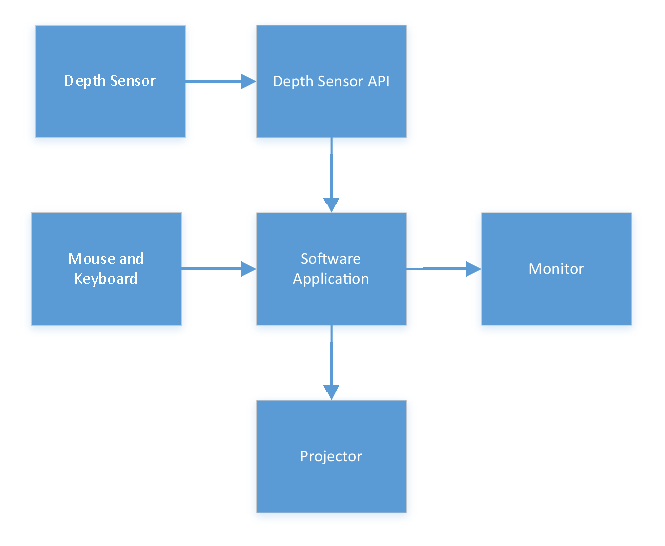
\includegraphics[width=6in]{BlockDiagram}
\end{center}

\pagebreak

\section{AR Sandbox Diagram}
The following diagram give a general idea of the hardware configuration of the AR sandbox.
\begin{center}
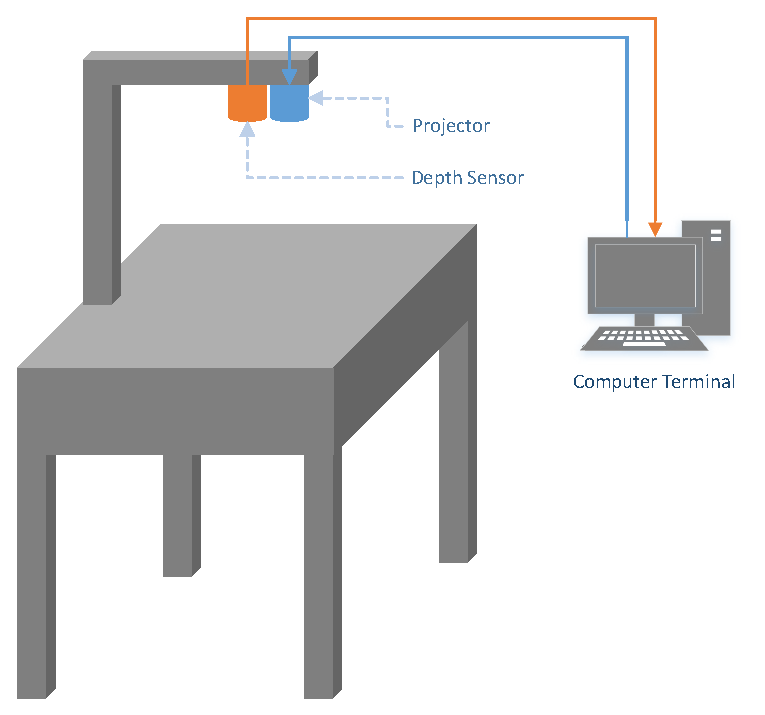
\includegraphics[width=6in]{Diagram}
\end{center}

\end{appendices}


\end{document}